\subsection{UC23 - Prenotazione tavolo}\label{usecase:23}

\begin{figure}[H]
  \centering
  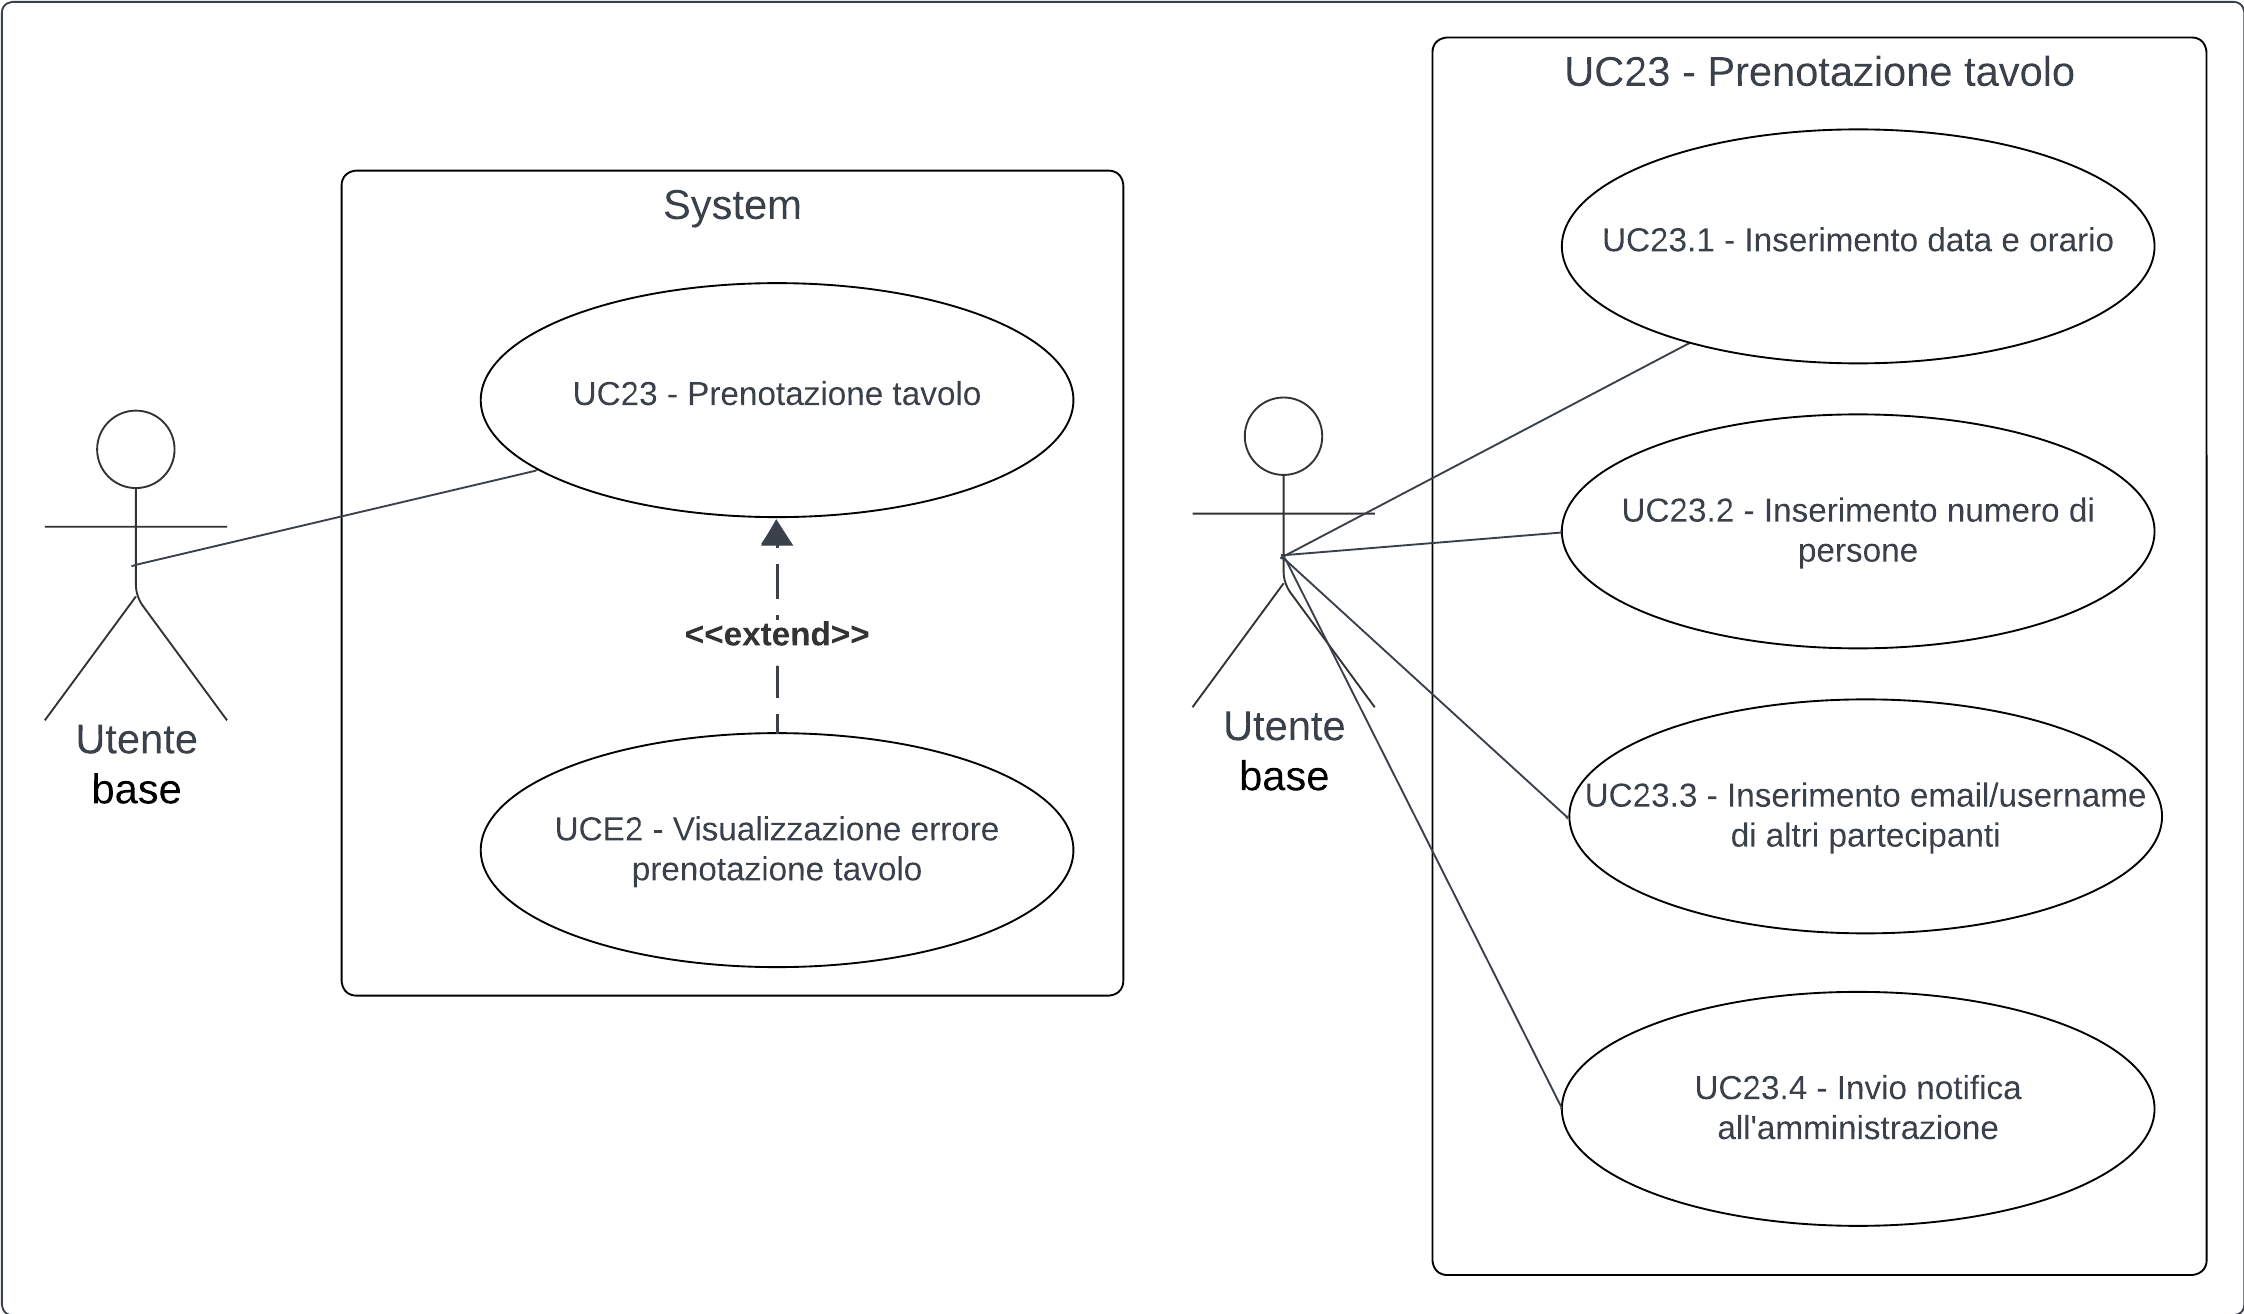
\includegraphics[width=0.9\linewidth]{ucd/UCD23.png}
\end{figure}

\textbf{Attori principali}:
\begin{itemize}
    \item Utente base autenticato
\end{itemize}
\textbf{Precondizione}:
\begin{itemize}
    \item L'utente è autenticato ed è riconosciuto come utente base
    \item L'utente ha già selezionato il ristorante tramite la ricerca ristorante \nameref{usecase:24}
\end{itemize}
\textbf{Postcondizione}:
\begin{itemize}
    \item L'utente ha richiesto una $\textit{Prenotazione}_G$ in un ristorante
    \item Il $\textit{Sistema}_G$ ha inviato una notifica al ristorante selezionato
\end{itemize}
\textbf{Trigger}:
\begin{itemize}
    \item L'utente vuole prenotare un tavolo nel ristorante selezionato
\end{itemize}
\textbf{Scenario principale}:
\begin{enumerate}
    \item L'utente inserisce nella query di ricerca la data.
    \item L'utente specifica l'orario di arrivo.
    \item L'utente specifica il numero di persone.
    \item L'utente specifica, inserendo username/email utente, chi sono le altre persone al tavolo.
    \item Il $\textit{Sistema}_G$ invia una notifica di una richiesta di $\textit{Prenotazione}_G$ agli amministratori del ristorante.
\end{enumerate}
\textbf{Scenari alternativi}:
\begin{itemize}
    \item Se si verifica:
    \begin{enumerate}
        \item L'utente decide di cancellare la prenotazione.
        \item Il ristorante non possiede tavoli liberi all'ora scelta.
        \item Il ristorante non possiede abbastanza posti per quell'ora.
    \end{enumerate}
    \item L'utente visualizza un messaggio di errore
    \item La $\textit{Prenotazione}_G$ viene cancellata
\end{itemize}



\subsubsection{UC23.1 - Inserimento data e ora}\label{usecase:23_1}
\textbf{Attori}:
\begin{itemize}
    \item Utente base autenticato
\end{itemize}
\textbf{Precondizioni}:
\begin{itemize}
    \item L'utente è autenticato ed è riconosciuto come utente base.
    \item L'utente ha già selezionato il ristorante tramite la ricerca ristorante \nameref{usecase:24}
\end{itemize}
\textbf{Postcondizioni}:
\begin{itemize}
    \item L'utente ha inserito correttamente la data e l'orario di arrivo per la prenotazione
\end{itemize}
\textbf{Scenario principale}:
\begin{enumerate}
    \item L'utente inserisce la data desiderata per la $\textit{Prenotazione}_G$ nel formato appropriato
    \item L'utente specifica l'orario di arrivo previsto nel formato appropriato.
\end{enumerate}



\subsubsection{UC23.2 - Inserimento numero di persone}\label{usecase:23_2}
\textbf{Attori}:
\begin{itemize}
    \item Utente base autenticato
\end{itemize}
\textbf{Precondizioni}:
\begin{itemize}
    \item L'utente è autenticato ed è riconosciuto come utente base.
    \item L'utente ha già selezionato il ristorante tramite la ricerca ristorante \nameref{usecase:24}
\end{itemize}
\textbf{Postcondizioni}:
\begin{itemize}
    \item L'utente ha inserito correttamente il numero di persone per la prenotazione.
\end{itemize}
\textbf{Scenario principale}:
\begin{enumerate}
    \item L'utente specifica il numero di persone che parteciperanno alla prenotazione.
\end{enumerate}


\subsubsection{UC23.3 - Inserimento email/username di altri partecipanti}\label{usecase:23_3}
\textbf{Attori}:
\begin{itemize}
    \item Utente base autenticato
\end{itemize}
\textbf{Precondizioni}:
\begin{itemize}
    \item L'utente è autenticato ed è riconosciuto come utente base.
    \item L'utente ha già selezionato il ristorante tramite la ricerca ristorante \nameref{usecase:24}
\end{itemize}
\textbf{Postcondizioni}:
\begin{itemize}
    \item L'utente ha inserito correttamente le informazioni degli altri partecipanti alla prenotazione.
\end{itemize}
\textbf{Scenario principale}:
\begin{enumerate}
    \item L'utente specifica, inserendo l'username/email degli altri partecipanti al tavolo, chi sono le altre persone coinvolte nella prenotazione.
\end{enumerate}


\subsubsection{UC23.4 - Invio notifica all'amministratore
}\label{usecase:23_4}
\textbf{Attori}:
\begin{itemize}
    \item Utente base autenticato
\end{itemize}
\textbf{Precondizioni}:
\begin{itemize}
    \item L'utente è autenticato ed è riconosciuto come utente base.
    \item L'utente ha già selezionato il ristorante tramite la ricerca ristorante \nameref{usecase:24}
    \item L'utente ha inserito correttamente tutte le informazioni necessarie per la prenotazione.
\end{itemize}
\textbf{Postcondizioni}:
\begin{itemize}
    \item Il $\textit{Sistema}_G$ ha inviato una notifica di una richiesta di $\textit{Prenotazione}_G$ agli amministratori del ristorante selezionato.
\end{itemize}
\textbf{Scenario principale}:
\begin{enumerate}
    \item Dopo aver completato l'inserimento di tutte le informazioni richieste, il $\textit{Sistema}_G$ invia una notifica di una richiesta di $\textit{Prenotazione}_G$ agli amministratori del ristorante selezionato.
\end{enumerate}



\newpage